\documentclass[11pt]{beamer}
\usetheme{default}
\usepackage[utf8]{inputenc}
\usepackage[polish]{babel}
\usepackage[T1]{fontenc}
\usepackage{amsmath}
\usepackage{amsfonts}
\usepackage{amssymb}
\author{Alan Andrzejak, Aleksy Dziarmaga, Michał Kloc}
\title{08. Mobilna edukacja: wykład oraz kolokwium w postaci testu jednokrotnego wyboru - projekt}
%\setbeamercovered{transparent}
\setbeamertemplate{navigation symbols}{}
\date{}
\subject{Quiz}
%%%%%%%%%%%%%%%%
\begin{document}
%%%
\begin{frame}
\titlepage
\end{frame}
%%%
\section{Plan prezentacji}
\begin{frame}
\frametitle{Plan prezentacji}\pause
\begin{itemize}
\item Cel aplikacji\pause
\item Wygląd aplikacji\pause
\item Baza pytań\pause
\item Stan projektu obecnie\pause
\item Możliwości rozwoju
\end{itemize}
\end{frame}
%%%
\section{Cel aplikacji}
\begin{frame}
\frametitle{Cel aplikacji}\pause
Zapewnienie:\\
\begin{itemize}
\item możliwości nauki mobilnej.\\\pause
\item import własnej bazy pytań.
\end{itemize}
\end{frame}
%%%
\section{Wygląd aplikacji}
\begin{frame}
\frametitle{Wygląd aplikacji}
Quiz:\pause
\begin{center}
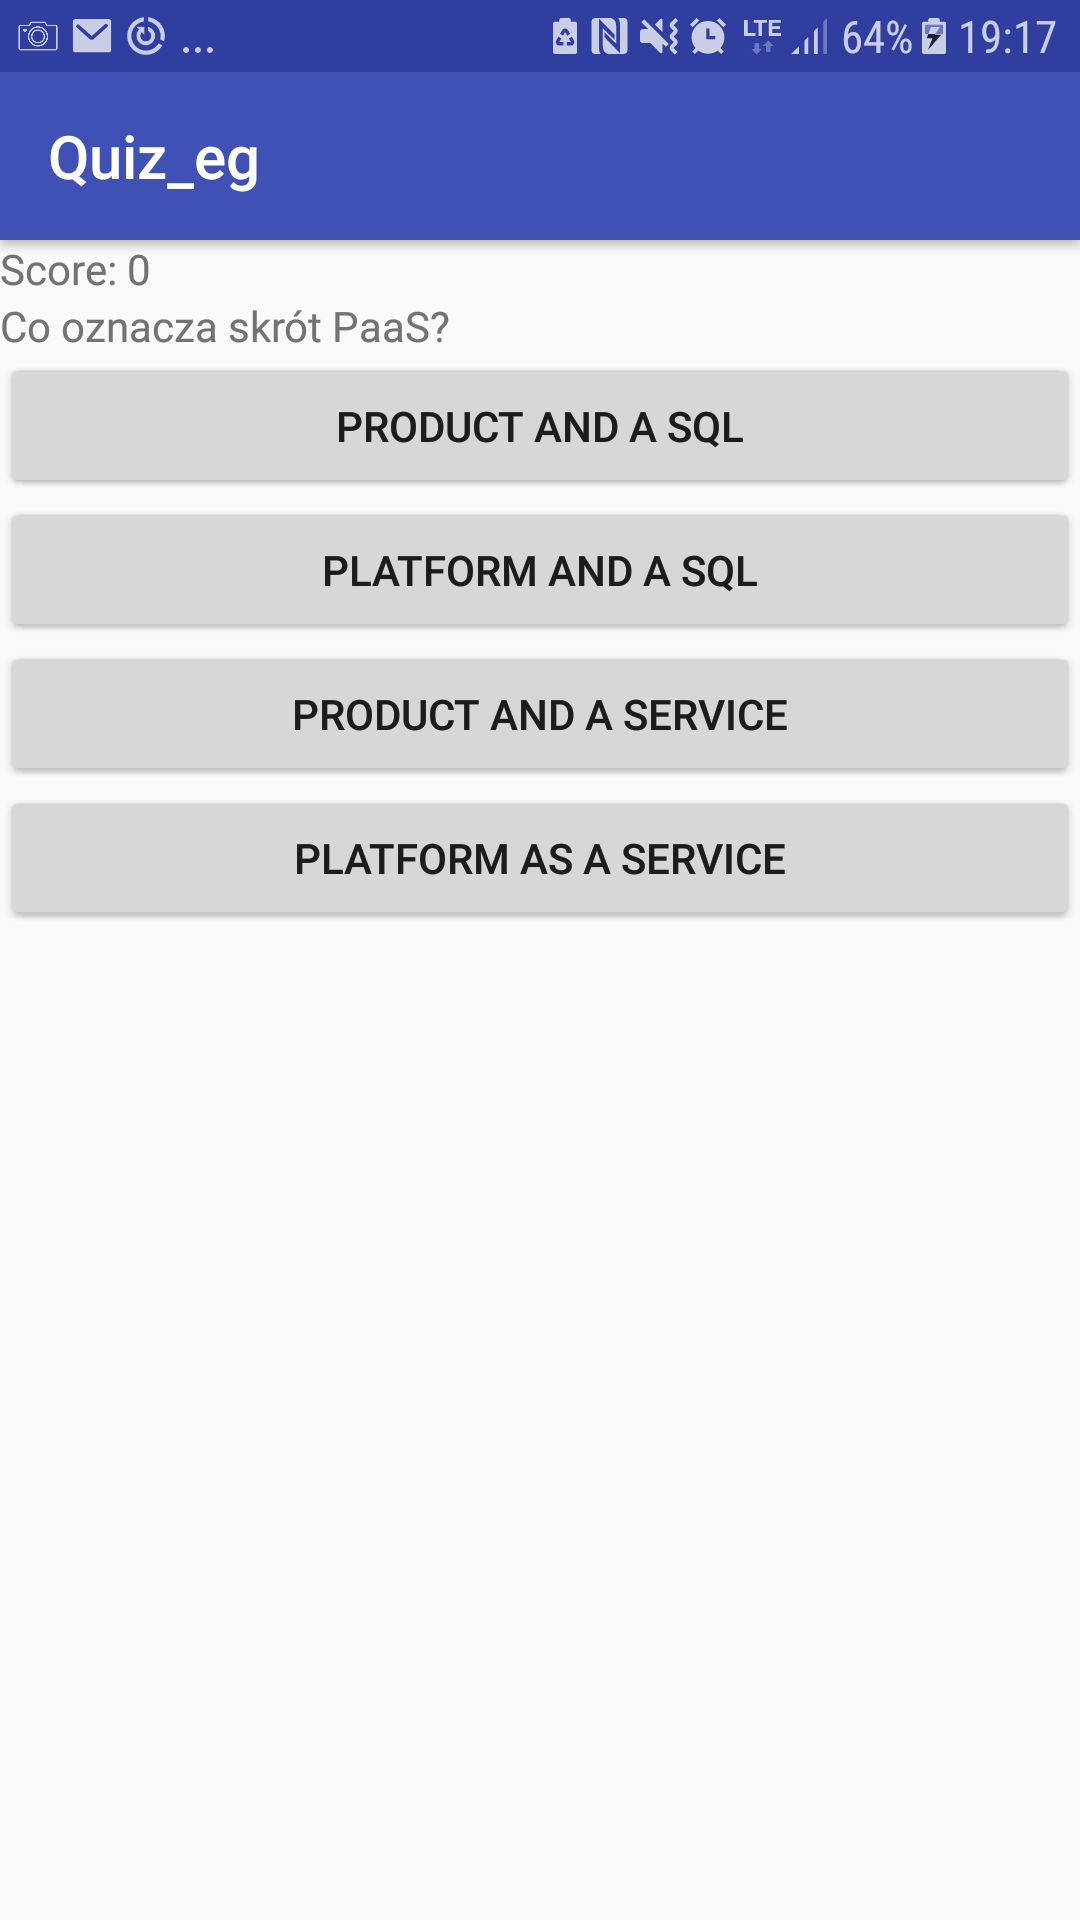
\includegraphics[scale=0.2]{../imgs/Quiz1_screenshot.png}
\end{center}
\end{frame}
%%%
\begin{frame}
\frametitle{Wygląd aplikacji}
Quiz:
\begin{center}
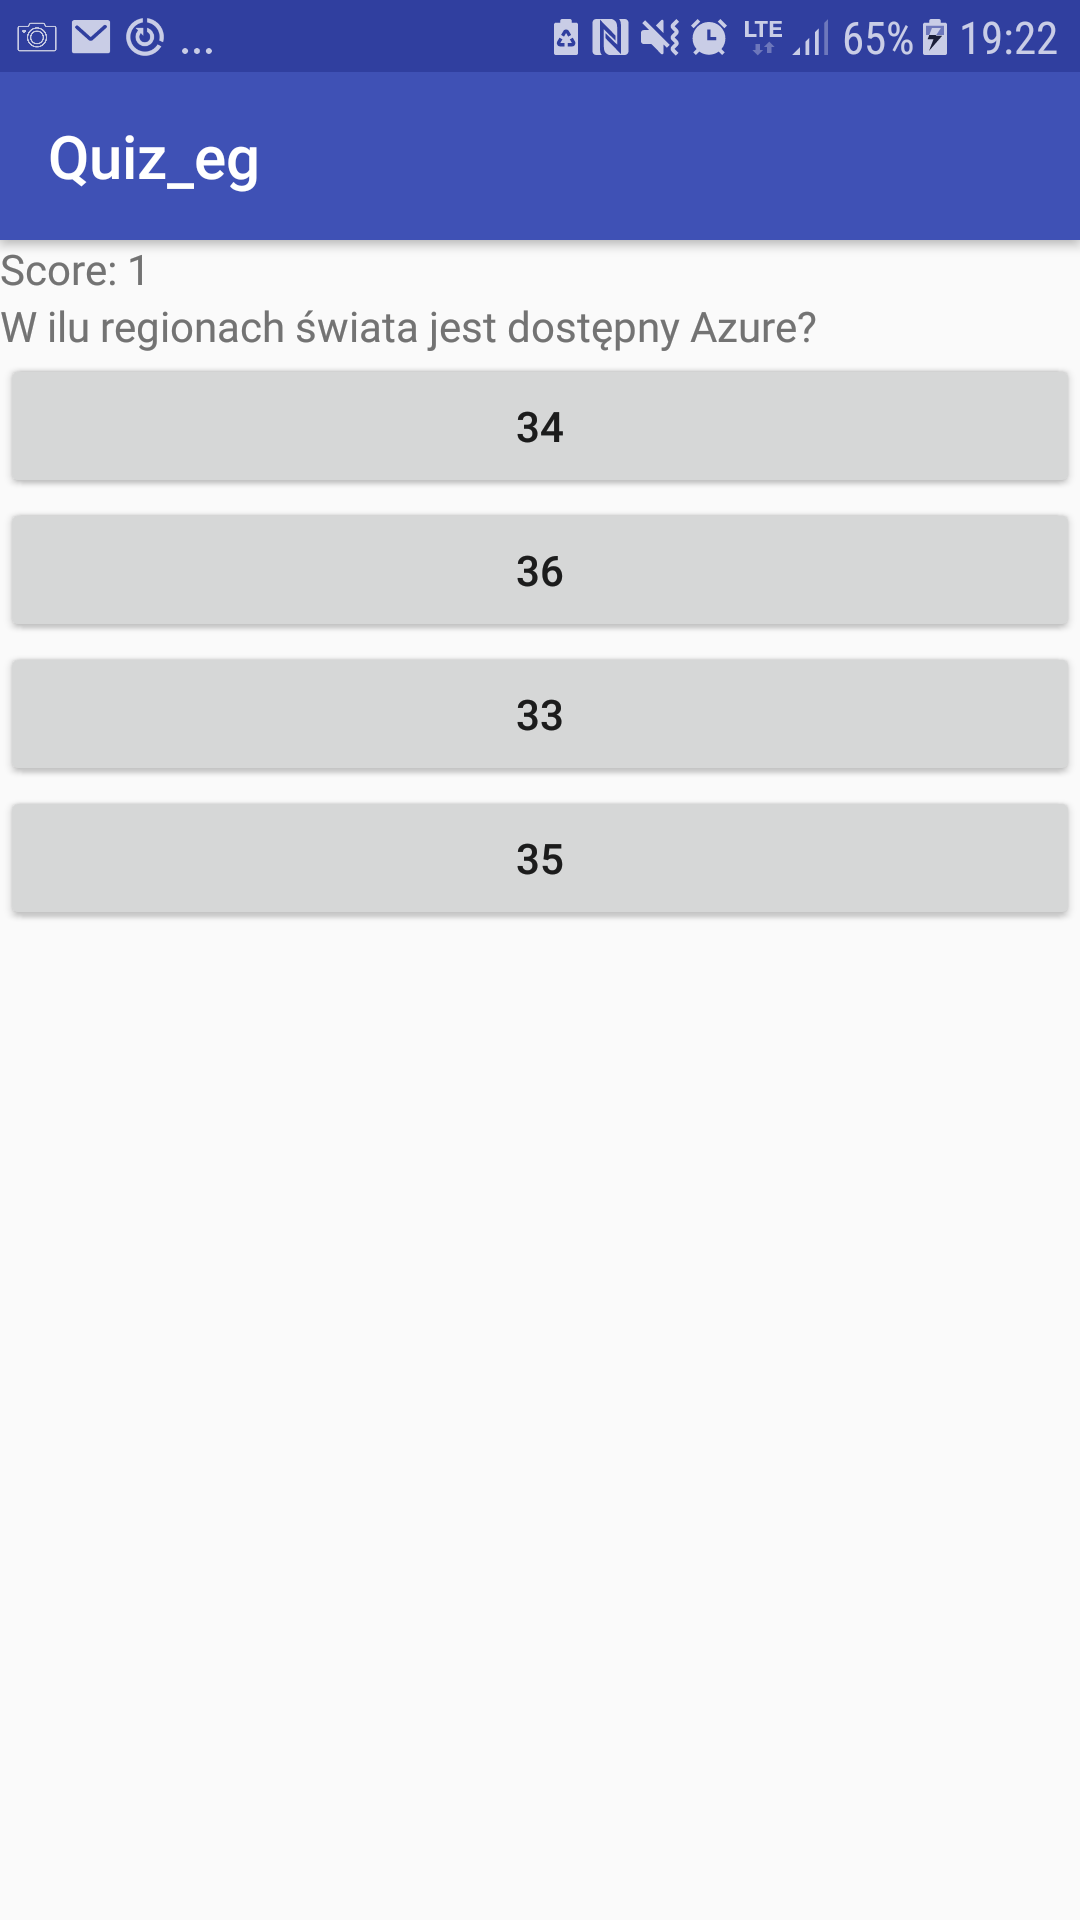
\includegraphics[scale=0.2]{../imgs/Quiz2_screenshot.png}
\end{center}
\end{frame}
%%%
\begin{frame}
\frametitle{Wygląd aplikacji}
Zakończenie quizu:
\begin{center}
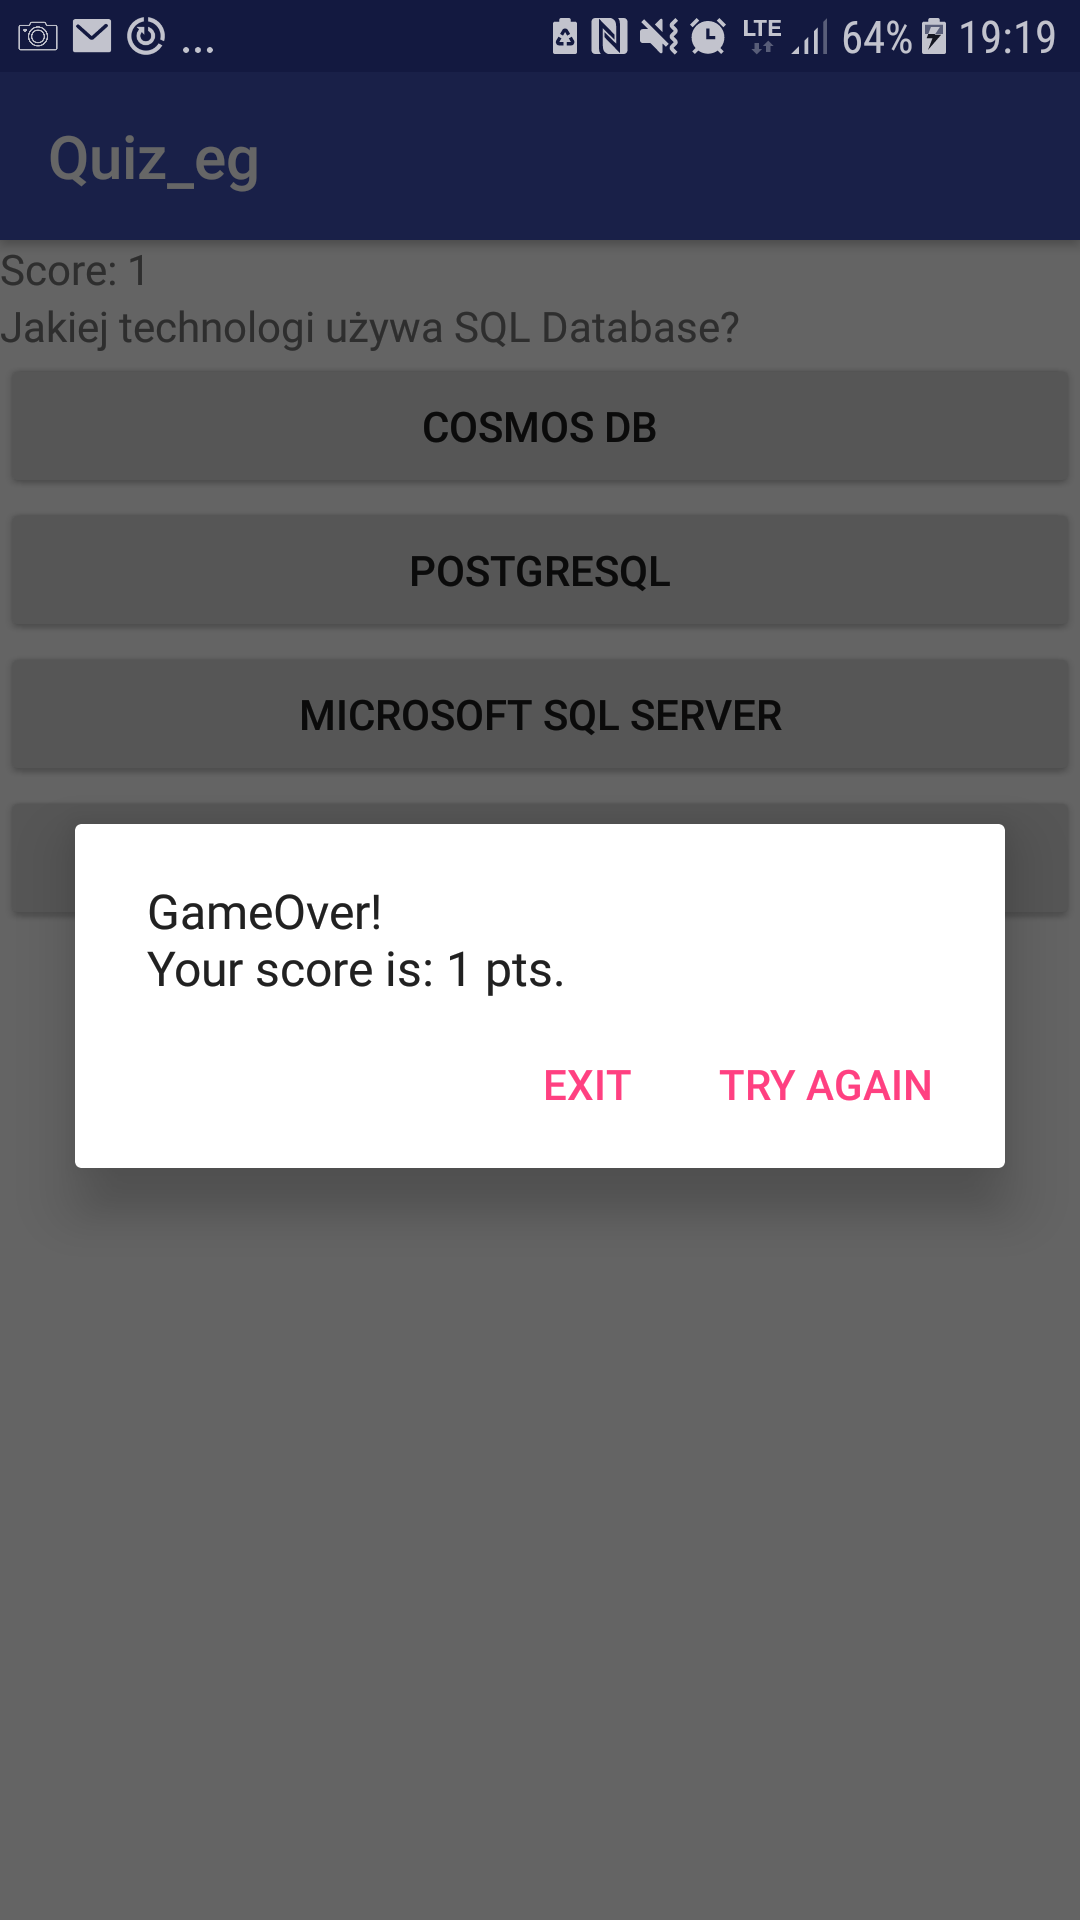
\includegraphics[scale=0.15]{../imgs/QuizOver_screenshot.png}
\end{center}
\end{frame}
%%%
\section{Baza pytań}
\begin{frame}
\frametitle{Baza pytań}
Przykładowy plik .xml:
\begin{center}
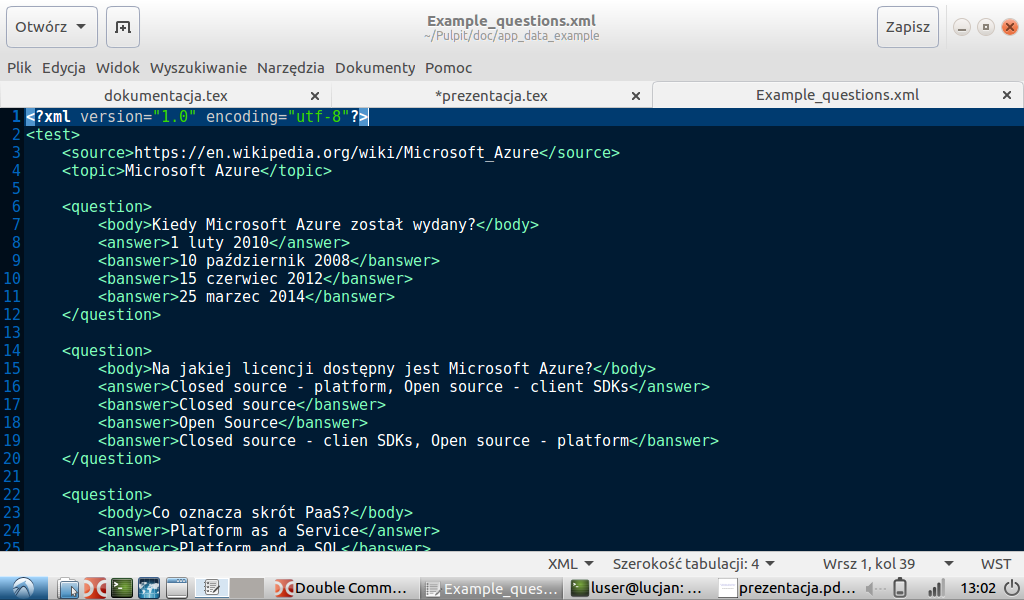
\includegraphics[scale=0.3]{../imgs/Xml_screenshot.png}
\end{center}
\end{frame}
%%%
\section{Stan projektu obecnie}
\begin{frame}
\frametitle{Stan projektu obecnie}\pause
Wykonano:\pause
\begin{itemize}
\item prosty layout\pause
\item wczytywanie pytań z baz/y w formacie .xml\pause
\item losowanie kolejności pytań i odpowiedzi\pause
\item quiz himself
\end{itemize}
\end{frame}
%%%
\section{Możliwości rozwoju}
\begin{frame}
\frametitle{Możliwości rozwoju}\pause
\begin{itemize}
\item dodać menu z możliwością konfiguracji quizu\pause
\item możliwość powrotu do poprzedniego pytania wraz z zapamiętaną odpowiedzią\pause
\item możliwość zapamiętania wyniku\pause
\item uzupełnić parser o ładowanie informacji dodatkowych\pause
\item różna ilość poprawnych i błędnych odpowiedzi
\end{itemize}
\end{frame}
%%%
\section{Podziękowania}
\begin{frame}
\frametitle{Podziękowania}\pause
\Huge{Dz\pause i\pause ęku\pause ję}
\end{frame}
%%%
\end{document}
%%%%%%%%%%%%%%%%
